\documentclass{beamer}

\usepackage{polski}
\usepackage[utf8]{inputenc}
\usepackage{color}
\usepackage{amsfonts}	% Real

\usepackage{booktabs} % eleganckie tabelki


\usetheme{boxes}      % Wybór tematu wyglądu, gdy chcemy inny
%\usecolortheme{rose}   % Wybór tematu kolorystycznego, j.w.

%Konfiguracja dla pakietu hyperref:
\hypersetup{
  unicode=true,           % włączenie wyświetlania pliterek w zakładkach
%  pdfpagemode=FullScreen, % włączenie trybu pełnoekranowanego
  pdfsubject=Graph Neural Networks,      % temat prezentacji
  pdfkeywords={gnn, graph neural network, graph, classification} % slowa kluczowe
}

%% Dane do strony tytułowej
\author{Aleksy Barcz\\mgr inż. Zbigniew Szymański, II PW}
\title{Graph Neural Networks}
%\date{\today}
%\institute{Institute of Computer Science \\ Warsaw University of Technology}

\setbeamercovered{transparent}

\begin{document}
\frame{\titlepage}

\begin{frame}
\frametitle{Plan prezentacji}
\begin{enumerate}
	\item Po co nam klasyfikacja grafów?
	\item Metody przetwarzania grafów
	\item Graph Neural Networks
	\item Wyniki
\end{enumerate}
\end{frame}

\begin{frame}
\frametitle{Zastosowania klasyfikacji grafów}
\begin{itemize}
	\item chemia
	\item klasyfikacja tekstu
	\item rozpoznawanie obrazów (RAG i in.)
	\item lokalizacja twarzy
	\item ranking stron WWW
\end{itemize}
\end{frame}

\begin{frame}
\frametitle{Po co nam klasyfikacja grafów?}
\begin{center}
	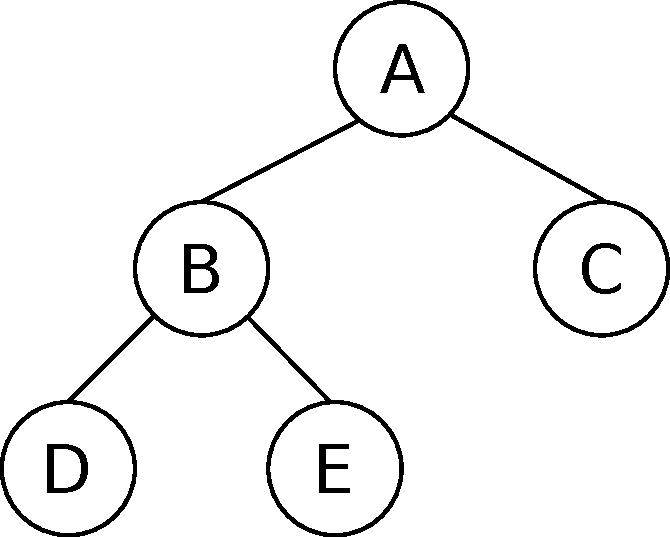
\includegraphics[scale=0.4]{img/tree}
\end{center}
Reprezentacja BFS: $[A, B, C, D, E]$
\begin{itemize}
	\item problem sąsiedztwa
	\item zależności cykliczne
	\item etykiety krawędzi
\end{itemize}
\end{frame}

\begin{frame}
\frametitle{Zadania klasyfikacji grafów}
\begin{itemize}
	\item budowanie reprezentacji danych
	\item klasyfikacja danych
\end{itemize}
\end{frame}

\begin{frame}
\frametitle{Metody klasyfikacji grafów}
\begin{itemize}
	\item funkcje jądra dla klasycznych klasyfikatorów
	\item metody probabilistyczne: sieci Bayesowskie i sieci Markowa
	\item metody oparte na sieciach neuronowych
\end{itemize}
\end{frame}

\begin{frame}
\frametitle{Metody oparte na sieciach neuronowych - historia}
\begin{itemize}
	\item 1943 - 1988 rozwój klasycznych sieci neuronowych (FNN)
	\item ...
	\item 1987 Rekurencyjne sieci neuronowe (RNN)
	\item ...
	\item 1990 RAAM (Pollack)
	\item 1993 LRAAM (Sperduti)
	\item 1997 Neuron rekurencyjny (Sperduti, Starita)
	\item 2005 Graph Machines (Goulon, Duprat, Dreyfus)
	\item 2009 Graph Neural Networks (Scarselli et al.)
\end{itemize}
\end{frame}

\begin{frame}
\frametitle{Cel pracy - implementacja GNN}
\begin{itemize}
	\item Implementacja GNN w oparciu o dostępne publikacje
	\item Identyfikacja kluczowych parametrów
	\item Odkrycie ograniczeń modelu
	\item Utworzenie wygodnego i uniwersalnego środowiska
\end{itemize}
\end{frame}

\begin{frame}
\frametitle{Cechy GNN}
\begin{itemize}
	\item Klasyfikator dowolnych grafów (niepozycyjne, cykle)
	\item Klasyfikacja węzłów oraz klasyfikacja grafów
	\item Oparty na FNN
	\item Budowanie reprezentacji jednoczesne z nauką klasyfikatora
\end{itemize}
\end{frame}

\begin{frame}
\frametitle{Przykładowy graf}
\begin{center}
	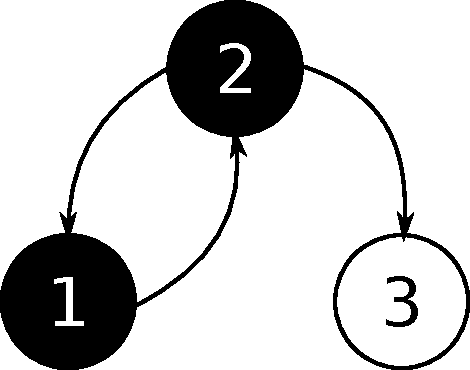
\includegraphics[scale=0.6]{img/graph_classes}
\end{center}
\begin{itemize}
	\item wierzchołki czarne - wartość oczekiwana +1
	\item wierzchołki białe - wartość oczekiwana -1
\end{itemize}
\end{frame}

\begin{frame}
\frametitle{Sieć kodująca}
\begin{center}
	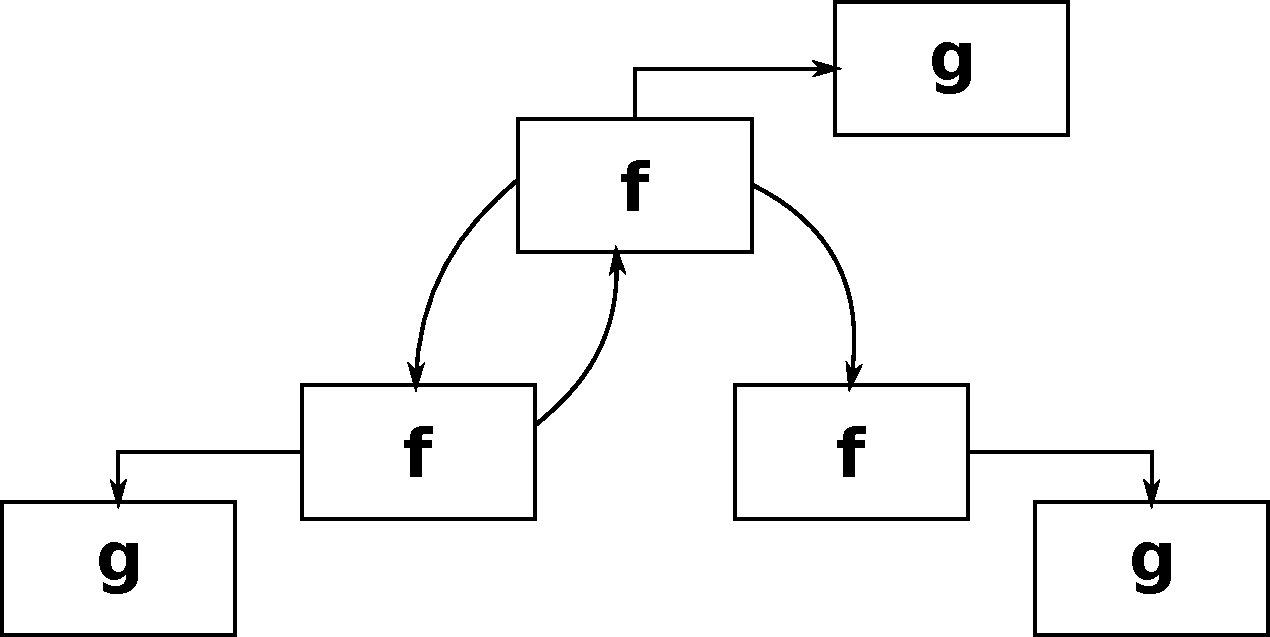
\includegraphics[scale=0.5]{img/encoding}
\end{center}
\begin{itemize}
	\item Dla każdego węzła budowana reprezentacja: $x_n = f(...)$
	\item Klasyfikacja węzła: $o_n = g(x_n)$
	\item Wszystkie instancje $f_w$ współdzielą wagi
	\item Wszystkie instancje $g_w$ współdzielą wagi
\end{itemize}
\end{frame}

\begin{frame}
\frametitle{Schemat uczenia GNN}
Algorytm:
\begin{enumerate}
	\item Losowa inicjalizacja stanu $X$
	\item do osiągnięcia kryterium stopu:
	\begin{itemize}
		\item FORWARD : obliczanie $X = F_w(X)$ aż do osiągnięcia punktu stałego
		\item BACKWARD : obliczenie $G_w(X)$ i propagacja wsteczna błędu
		\item aktualizacja wag $f_w$ i $g_w$
	\end{itemize}
\end{enumerate}
\end{frame}

\begin{frame}
\frametitle{Forward - budowanie stanu}
\begin{columns}
	\begin{column}{0.66\textwidth}
		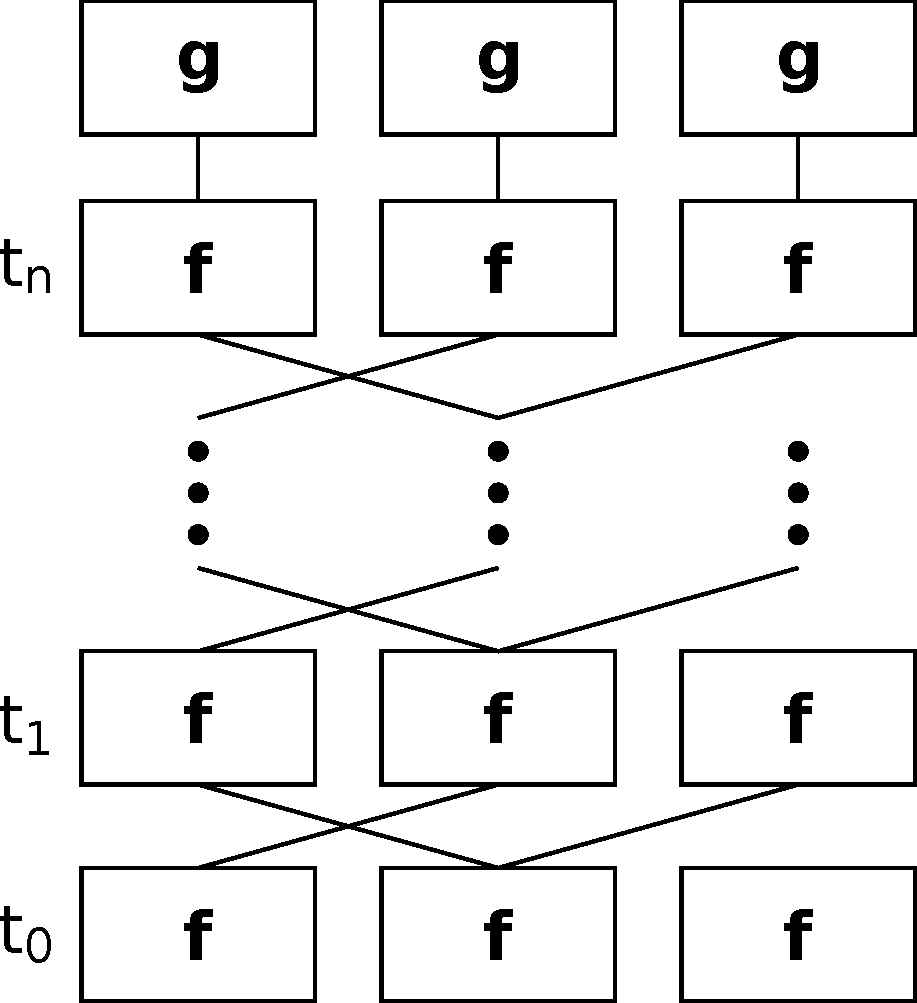
\includegraphics[scale=0.4]{img/forward}
	\end{column}
	\begin{column}{0.34\textwidth}
		\begin{itemize}
			\item BPTT
			\item $minStateDiff$
		\end{itemize}
	\end{column}
\end{columns}
\end{frame}

\begin{frame}
\frametitle{Backward - propagacja wsteczna błędu}
\begin{columns}
	\begin{column}{0.66\textwidth}
		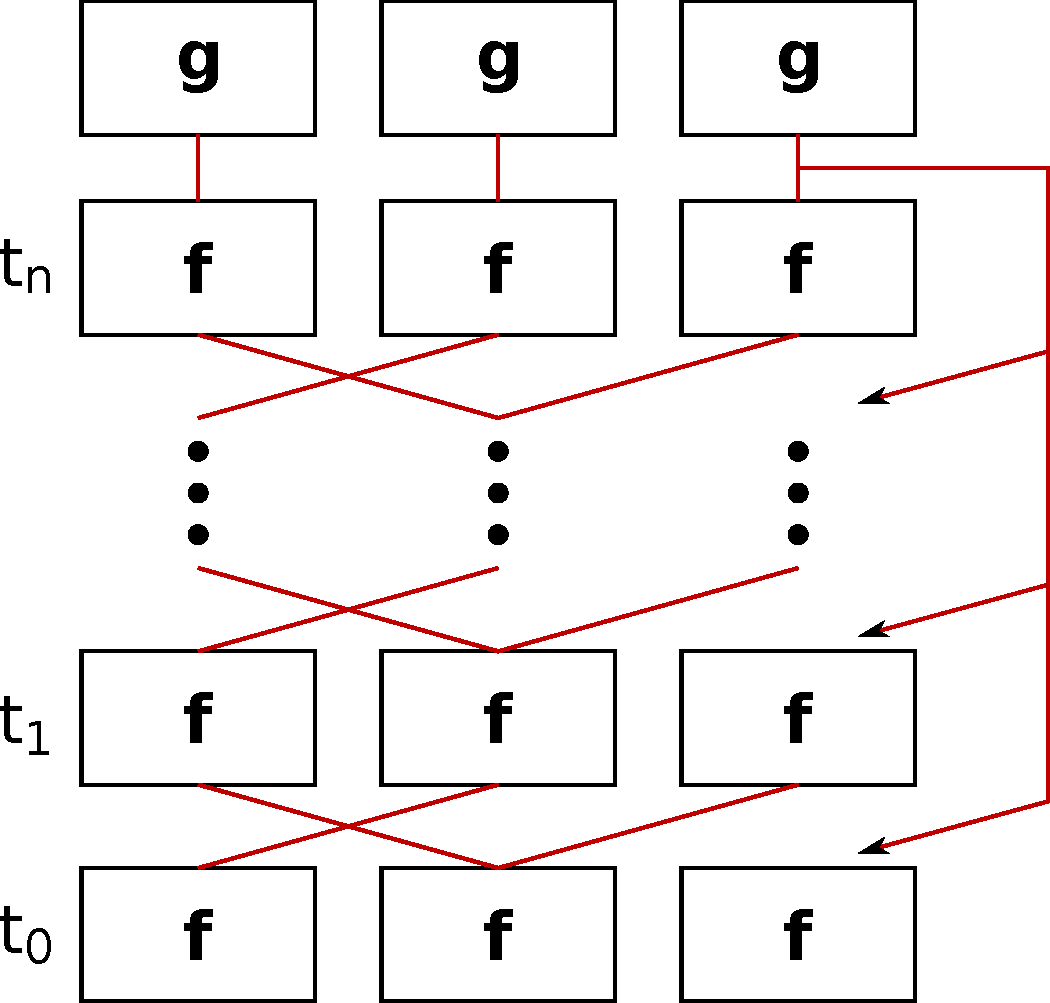
\includegraphics[scale=0.4]{img/backward}
	\end{column}
	\begin{column}{0.34\textwidth}
		\begin{itemize}
			\item Almeida-Pineda
			\item $minErrorDiff$
		\end{itemize}
	\end{column}
\end{columns}
\end{frame}

\begin{frame}
\frametitle{Skąd wiemy że $F_w$ jest zbieżna?}
\begin{itemize}
	\item odwzorowanie zwężające (tw. Banacha)
	\item kara nakładana na wagi w przypadku utraty tej właściwości
\end{itemize}
\end{frame}

\begin{frame}
	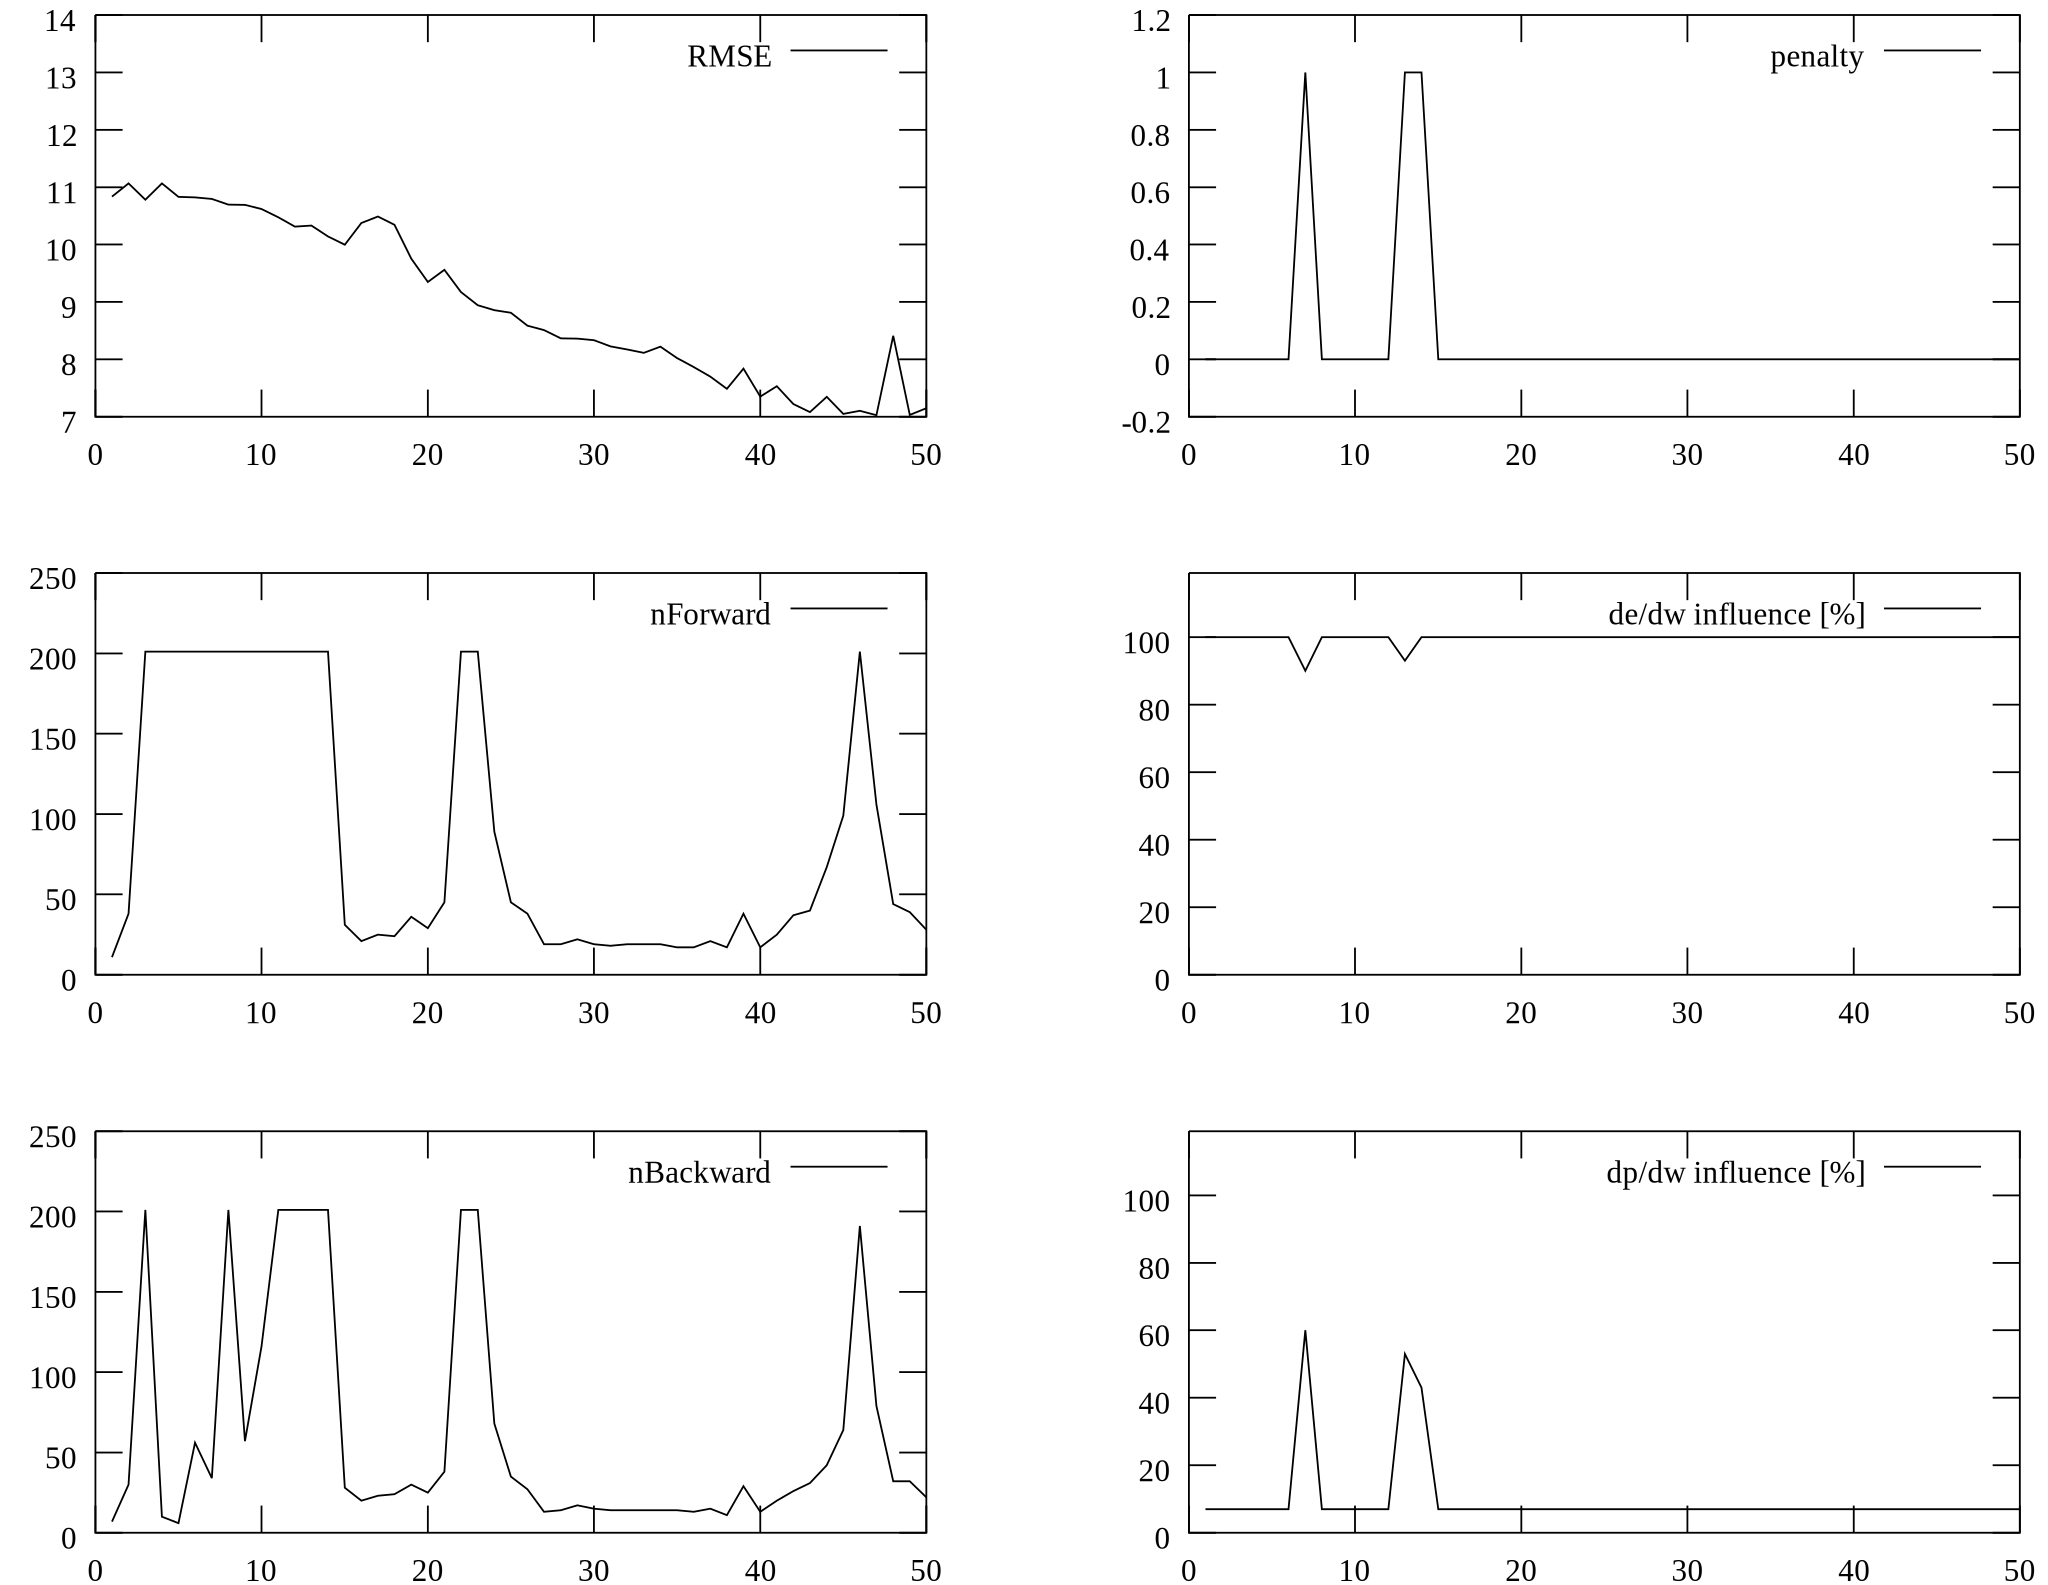
\includegraphics[scale=0.065]{img/params_set3}
\end{frame}

\begin{frame}
\frametitle{Porównanie FNN/GNN}
\begin{itemize}
	\item 14 węzłów, 7 węzłów podgrafu
	\item FNN : najlepsza z 10ciu, 5-krotna walidacja krzyżowa
	\item GNN : losowa sieć, 5-krotna walidacja krzyżowa, 50 iteracji
\end{itemize}
\end{frame}

\begin{frame}
\frametitle{Wyniki}
\setlength{\tabcolsep}{2pt}
\begin{table}[h!]
	\begin{center}
	\begin{tabular}{llll}
	\toprule
	& accuracy & precision & recall \\
	\midrule
	FNN - tr &	71\% &  65\% & 93\% \\
	FNN - tst &	71\% &  64\% &  93\% \\
	GNN - tr &	91\% &  87\%&  97\% \\
	GNN - tst &	91\% &  86\% &  97\% \\
	\bottomrule
	\end{tabular}
	\caption{Średnie wartości na zbiorze uczącym i testowym}
	\end{center}
\end{table}

\begin{table}[h!]
	\begin{center}
	\begin{tabular}{llll}
	\toprule
	& accuracy & precision & recall \\
	\midrule
	FNN - tr &	0.34\% &  0.67\% & 1.86\% \\
	FNN - tst &	2.45\% &  1.73\% &  2.93\% \\
	GNN - tr &	1.62\% &  1.71\% &  2.07\% \\
	GNN - tst &	3.06\% &  3.70\% &  1.39\% \\
	\bottomrule
	\end{tabular}
	\caption{Odchylenia standardowe}
	\end{center}
\end{table}
\end{frame}

\end{document}
